\documentclass[a4paper,12pt]{report}

\usepackage{amsmath,amsfonts,mathtools}
\usepackage{hyperref}

\usepackage{listings}
\usepackage{color}

\definecolor{dkgreen}{rgb}{0,0.6,0}
\definecolor{gray}{rgb}{0.5,0.5,0.5}
\definecolor{mauve}{rgb}{0.58,0,0.82}

\begin{document}
\title{ECE253 Abridged}
\author{Aman Bhargava}
\date{September 2019}
\maketitle

\tableofcontents

\pagebreak

\chapter{Review: Bit Manipulation}
Have you ever wanted to be a cool computer person who does things with ones and zero's instead of actual letters and numbers like a normal person? If so, this is the right chapter for you!

\section{Converting to and from Different Bases}
Base 10, 2, and 16 are most commonly used. Base 16 is just a way to read base 2 in a more efficient manner. In order to work with bits it's pretty important to know how to convert back and forth because the test is all on paper. 

\subsection{Converting from base 10 $\to$ base 2}
You keep dividing by two, keeping track of the remainder. Eventually the number you will be trying to divide by two will be 1. You keep going until it's zero + remainder(1). Then you read the reaminders upward from that final 1.

\subsection{Converting from base 2 $\to$ base 16}
Any hex number can be expressed as 4 binary digits. Make a correspondence table between quadruplets of binary numbers and hex (1-f, inclusive). To convert to base 16 subdivide from right to left in groups of four binary digits. Pad the leftmost part with leading zeros and convert using the table. 

\subsection{Converting from base 10 $\to$ base 16 (and vice versa)}
Just go through base 2 fam.

% \chapter{Logic Functions and Logic Gates}
% \section{Or Gate}
% \begin{enumerate}
% \item Symbols
% \item Switch structure
% \item Truth table
% \end{enumerate}

% \section{And Gate}

% \section{Inverter}

% \section{XOR}


\chapter{Boolean Algebra}
Here are the axioms of Boolean Algebra:
\begin{enumerate}
\item $0 \cdot 0 = 0$
\item $1 \cdot 1 = 1$
\item $0 \cdot 1 = 1 \cdot 0 = 0$
\item if $x = 0$, $!x = 1$
\end{enumerate}

\paragraph{Dual Form}
\begin{enumerate}
\item $1 + 1 = 1$
\item $0 + 0 = 0$
\item $1 + 0 = 0 + 1 = 1$
\item if $x = 1$, $!x = 0$
\end{enumerate}

\paragraph{Duality: } In a given logic expression, you can swap $1 \to 0$ and $\cdot \to +$
and the expression is still valid.

\section{Useful Boolean Expression Rules}
\begin{itemize}
\item $x \cdot 0 = 0$
\item $x \cdot 1 = x$
\item $x \cdot x = x$
\item $x \cdot !x = 0$
\item $x \cdot 0 = 0$
\item $!!x = x$
\item $x + 1 = 1$
\item $x + 0 = x$
\item $x + x = x$
\item $x + !x = 1$
\end{itemize}

\paragraph{Distributive Properties: }
$$x \cdot (y + z) = xy + xz$$
$$x + (y \cdot z) = (x+y) \cdot (x+z)$$

% \section{Less Obvious Identities}
% \begin{itemize}
% \item 
% \end{itemize}


\section{Sum-of-Products (SOP)}
'Sum' means boolean OR while 'product' means boolean AND. 

\paragraph{Min term: } for $n$ variables, term where all variables appear once is a 'minterm'.
Note that variables can either be complimented or uncomplimented. 

Any boolean function can be represented by the sum of products of minterms - this is just done 
by simply converting the truth table and OR-ing each truth. 

Then, you can simplify. Pretty common sense. 'Canonical' just means it's a bunch of midterms
separated by OR's.

\section{Product of Sums (POS)}
\paragraph{Max term: } where all $n$ variables appear OR-d. They can be complimented or
un-complimented. 

You can pretty easily make all the valid max terms from a truth table. To generate a POS
expression, you multiply (AND) the maxterms that sum to zero. 

% \section{NAND and NOR Logic Networks (TB 2.7)}


% \section{Three-Way Light Control (TB 2.8.1)}


\chapter{How 2 Verilog}
A 3-input multiplexer can be made with two 2-input multiplexers.
Now let's implement this without using two pre-made multiplexers. Let:
\begin{itemize}
\item 
\end{itemize}

\paragraph{Notes on Implementation}
\begin{itemize}
\item If you want inputs to be registered from switches, you need to assign them SW[<int>]
\item Likewise, if you want outputs to be registered to LED's, assign them LEDR[<int>]
\end{itemize}

\subsection{Code: 3-Way Multiplexer}

\lstset{frame=tb,
  language=Verilog,
  aboveskip=3mm,
  belowskip=3mm,
  showstringspaces=false,
  columns=flexible,
  basicstyle={\small\ttfamily},
  numbers=none,
  numberstyle=\tiny\color{gray},
  keywordstyle=\color{blue},
  commentstyle=\color{dkgreen},
  stringstyle=\color{mauve},
  breaklines=true,
  breakatwhitespace=true,
  tabsize=3
}

\begin{lstlisting}
module mux2b2to1 (SW, LEDR); //Two bit 2 to 1 multiplexer  
   input[4:0] SW, //[4:0] sets switches 0-4 to inputs(?)
   output[1:0] LEDR, //

   wire S;
   wire[1:0] a, b, z; //'two bit wide vector'?

   assign a = SW[1:0],
   assign b = SW[3:2],
   assign s = SW[4],
   assign LEDR = z,

   assign z[0] = (~s&a[0]) | (s&b[0]);
   assign z[1] = (~s & a[1]) | (s&b[1]);

endmodule;
\end{lstlisting}

\paragraph{Can you make the assignment more efficient?}
What if you do this:
\begin{lstlisting}
   // assign z[0] = (~s&a[0]) | (s&b[0]);
   // assign z[1] = (~s & a[1]) | (s&b[1]);
   assign z = (~s&a) | (s&b); // NOT CORRECT
\end{lstlisting}

\paragraph{Because $s$ is only 1-bit and $a, b$ are two bits, $s$ is extended with a \textbf{0}, 
which makes the logic incorrect!}

\paragraph{General Notes on how Syntax Works:}
\begin{itemize}
\item \textbf{What is 'assign'? } 'assign' just means you're making a connection (alias?) b/w the
two. \textbf{Question: } is this necessary for instantiating the variable?
\item \textbf{Assignment arith.} When you create a verilog wire/input with $x = [a:b]$, the number of bits in 
$x$ is $b-a + 1$
\item \textbf{Bit Access: } To access bits, you say $x[n]$ or $x[n:m]$ where $n < m$. The length of the slice
is $n-m +1$
\item \textbf{Concatenation: } If you want to stitch together multiple bits, you use $x = {SW[9:8], SW[1:0]}$. That
statement stitches together two 2-bit chunks ($SW[9:8], SW[1:0]$ to make one 4-bit chunk).
\item \textbf{Order of Operations: } Basically nobody knows... just use parenthesis when you're
not sure. And goes before or, though.
\end{itemize}


\section{Full Adder}
\paragraph{Description: }
Adding in binary is the same as in decimal, just with fewer options. When adding two single bits,
we have three output possibilities: $00, 01, 10$. We call the least significant bit the sum $s$ and
the most significant digit the carry $c$.

Let's see the truth table:
\begin{tabular}{ll|ll}
$x$ & $y$ & $C$ & $s$ \\
\hline
0 & 0 & 0 & 0 \\
0 & 1 & 0 & 1 \\
1 & 0 & 0 & 1 \\
1 & 1 & 1 & 0 \\
\end{tabular}

As you can see, the sum bit is just $x \oplus y$ and the carry bit is $xy$. 
This is a \textbf{half adder} because it doesn't accept a carry from the last calculation.

A full adder accepts a carry in $C_{in}$, $x$, and $y$, and outputs sum $s$ and carry out $C_{out}$.

Let's see the truth table:
\begin{tabular}{lll|ll}
$x$ & $y$ & $C_{in}$ & $C_{out}$ & $s$ \\
\hline
0 & 0 & 0 & 0 & 0 \\
0 & 0 & 1 & 0 & 1 \\
0 & 1 & 0 & 0 & 1 \\
0 & 1 & 1 & 1 & 0 \\
1 & 0 & 0 & 0 & 1 \\
1 & 0 & 1 & 1 & 0 \\
1 & 1 & 0 & 1 & 0 \\
1 & 1 & 1 & 1 & 1 \\
\end{tabular}

Therefore $$C_{out} = xy + xC_{in} + yC_{in}$$
and $$s = x \oplus y \oplus C_{in}$$

\paragraph{Ripple Carry Adder: } Then you can string them together by assigning one of these 
adders to each bit of the output and passing the carry out to the carry in of the next bit!

\paragraph{Specifics for Ripple Carry Adder: }
\begin{itemize}
\item Max size for output is one more then the two input's sizes because one more order of 
magnitude in binary is just doubling the number, and the most you can do when adding two 
numbers of equal length is double them.
\item Basically just string them together and you're golden.
\end{itemize}

\paragraph{Review of Outcomes}
\begin{itemize}
\item $Cout = xy + CinX + CinY$
\item $Sum = x \oplus y \oplus z$
\end{itemize}

\paragraph{Now let's make it in verilog!}
\begin{lstlisting}
module fulladder(x, y, Cin, S, Cout);
   input x, y, Cin;
   output S, Cout;

   assign s = x ^ y ^ Cin;
   assign Cout = (x&y) | (Cin&x) | (Cin&y); // Why no wires here? Bc no physical IO's.
\end{lstlisting}

\paragraph{Now we make a 3-bit adder out of full adders in Verilog!}
\begin{lstlisting}
module adder3bit(X, Y, S)
   input[2:0] X, Y;
   output[3:0] S;
   wire[3:0] C; // to connect full adders together

   fulladder U0(X[0], Y[0], C[0], C[1]);
   fulladder U1(X[1], Y[1], C[1], C[2]);
   fulladder U2(X[2], Y[2], C[2], C[3]);

   assign S[3] = C[3]; // Final carry bit is the most significant bit of the sum.
   assign C[0] = 1'b0; // Weird syntax: 1 bit, equal to 0.
endmodule;
\end{lstlisting}

This is structural verilog - we can't immediately see the bigger picture. We see wires and 
modules stitched together and we have to figure out what it all means.

\paragraph{Weird constant syntax: }
\begin{itemize}
\item $1'b0$: 1 bit constant, in binary, equal to 0.
\item $4'hF$: 4 bit constant, in hex, equal to F.
\item $4'd9$: 4 bit constant, in decimal, equal to 9.
\item $8'h1E$: 8 bit constant, in hex, equal to 1E.
\end{itemize}

\section{7-Segment Display}
\paragraph{Prompt: } Design a c ircuit with two inputs $x_1$ and $x_0$ representing a 
2-bit number $x$. Show $x$ on the 7-segment display (ranges from 0-3 inclusive).

\paragraph{Numbering: } $h_0$ is the top segment. Clockwise increases. $h_6$ is the middle one.

\paragraph{Note on D1-SoC Board: } Logic 0 makes the light turn on for $h_{0-6}$ and 1 makes 
it turn off ('active low')

\subsection{Displaying Numbers}
Sections to light up for 0: $h_{0-5}$
Sections to light up for 1: $h_{1-2}$
Sections to light up for 2: $h_{0-1}, h_6, h_{3-4}$
Sections to light up for 3: $h_{0-3}, h_6$

\paragraph{With active low: }
Sections to power for 0: $h_{6}$
Sections to power for 1: $h_{0}, h_{3-6}$
Sections to power for 2: $.$
Sections to power for 3: 

\paragraph{Truth Table: }
\begin{tabular}{ll|lllllll}
$x_1$ & $x_2$ & $h_6$ & $h_5$ & $h_4$ & $h_3$ & $h_2$ & $h_1$ & $h_0$  \\
\hline
0 & 0 & 1 & 0 & 0 & 0 & 0 & 0 & 0  \\
0 & 1 & 1 & 1 & 1 & 1 & 0 & 0 & 1  \\
1 & 0 & 0 & 1 & 0 & 0 & 1 & 0 & 0  \\
1 & 1 & 0 & 1 & 1 & 0 & 0 & 0 & 0  \\
\end{tabular}

\paragraph{Consolidating the Logic Functions: }
$$h_0 = (!x_1) \cdot x_0$$
$$h_1 = 0$$
$$h_2 = x_1 \cdot !x_0$$
$$h_3 = !x_1 \cdot x_0$$
$$h_4 = x_0$$
$$h_5 = x_1 | x_0$$
$$h_6 = !x_1$$

\paragraph{Verilog Code: }
\begin{lstlisting}
module seg7(SW, HEX0)
   input[1:0] X;
   output[6:0] HEX0;
   
   assign HEX0[0] = ~SW[1] & SW[0];
   // etc.

endmodule
\end{lstlisting}

\paragraph{Implementation Example: }
Designa  circuit with 4 inputs $a, b, c, d$ and $s$. 
   if s = 0, show $a+b$ on 7-seg display
   if s = 1, show $c+d$ on 7-seg display

$${a, b} \to mux_{2 bit * 2 inputs} \to fulladd_{cin = 0} \to HEXO \to output$$

\begin{itemize}
\item The carry in digit to the full adder is 0
\item The carry out from the full adder is the most significant digit of the HEXO input.
\item Honestly you could just use a half adder because you don't need a carry-in. 
$C_{out} = xy$, $Sum = x \oplus y$
\end{itemize}

\paragraph{Cool XOR Fact: } $\oplus$ returns 1 if the number of true inputs is ODD.

\section{FPGA's}
Can do anything.
\begin{itemize}
\item Field programmable gate arrays: Programmable in the field (i.e. not in the factory necessarily).
\item 2-D array of programmable blocks.
\item Blocks contain lookup tables (LUT)
\item Any two input LUT can be programmed for any two-input logic functions.
\item More complex logic comes out when you connect the LUTS - this is what Quartus does. 
\end{itemize}

\paragraph{How to encode any two-input thing}
Let there be 4 sRAM bits $p, q, r, s$. Let the inputs be $a, b$. 

$${p, q} \to mux_{a1} \to x$$
$${r, s} \to mux_{a1} \to y$$
Where $x, y$ are itermediate variables.

$${x, y} \to mux_{b} \to output$$

Therefore it takes 4 ram cells for a 2-input LUT. $$n_{ramcells} = 2^{inputs}$$

There are 85,000 6-LUTS on lab chips.

\chapter{Karnaugh Maps}
\section{Motivation}
Creating boolean functions to get what you need done is confusing and unlikely to lead to an optimal solution 
when there are many variables.

Karnaugh maps are a tool for expressing your truth tables in such a way that makes getting optimal solutions easier
with many variables.

\paragraph{Example 2x2 Karnaugh Map}
\begin{tabular}{l|cc}
& $0$ & $1$ \\
\hline
0 & a & b \\
1 & c & d \\
\end{tabular}


\section{Review of Terminology}

\begin{itemize}
\item \textbf{Implicant:} Any product term for which the function is true (think 'implies' logic is 1)
\item \textbf{Cover:} A set of implicants that covers all 1's of the function.
\item \textbf{Prime implicant:} Any implicant that, if we delete a literal, is no longer an implicant (largest
   groups of ones in the K-map)
\item \textbf{Essential prime implicant:} Prime implicant that covers a 1 covered by no other prime implicant.
\item \textbf{Min-cost cover:}
\item \textbf{Cost:}
\end{itemize}

\paragraph{Example: }
\begin{tabular}{l|cccc}
& $00$ & $01$ & $11$ & $10$   \\
\hline
0 & 1 & 1 & 1 & 1 \\
1 & 1 & 0 & 0 & 0 \\
\end{tabular}

Let the left column be the $z$ column and the top be products of $x, y$. 

List of implicants:
\begin{enumerate}
\item $\bar{z}$ 
\item $\bar{x} \bar{y}$
\item $\bar{x} \bar{z}$
\item $y\bar{z}$
\item $x\bar{z}$
\item $\bar{y}\bar{z}$
\item $m_{0, 1, 2, 4, 5}$
\end{enumerate}

Prime Implicants: Largest group of ones in cardinal maps...

\paragraph{Cost Defininition: } $n_{gates} + n_{inputs}$

\section{Procedure for Minimum Cost Cover}
\begin{itemize}
\item Find essential prime implicants and include in cover
\item Select additional prime implicants to include in the cover until all 1's are covered.
\end{itemize}

\section{5 Variable Karnaugh Map}
Use two 4-variable K-Maps. One for case where $x_5 = 0$, other for $x_5 = 1$.
Min-term indexing goes by the binary representation of $x_{0-n}$ where $x_n$ is the LEAST significant bit.


\chapter{Storage Elements}
\section{Introduction}
Until now, the values coming in have dependend on the state (high or low) of the input 
wires to the circuit. There's another option where the inputs dependent on past states 
of the circuit.

\paragraph{Storage elements } represent a \textbf{state} of a circuit. When inputs 
change, new inputs either leave circuit in the same state or change the state. These 
circuits are called \textbf{sequential} circuits. Memory elements can be created 
with logic gates. 

\section{RS Latches}
\begin{figure}[h]
\centering
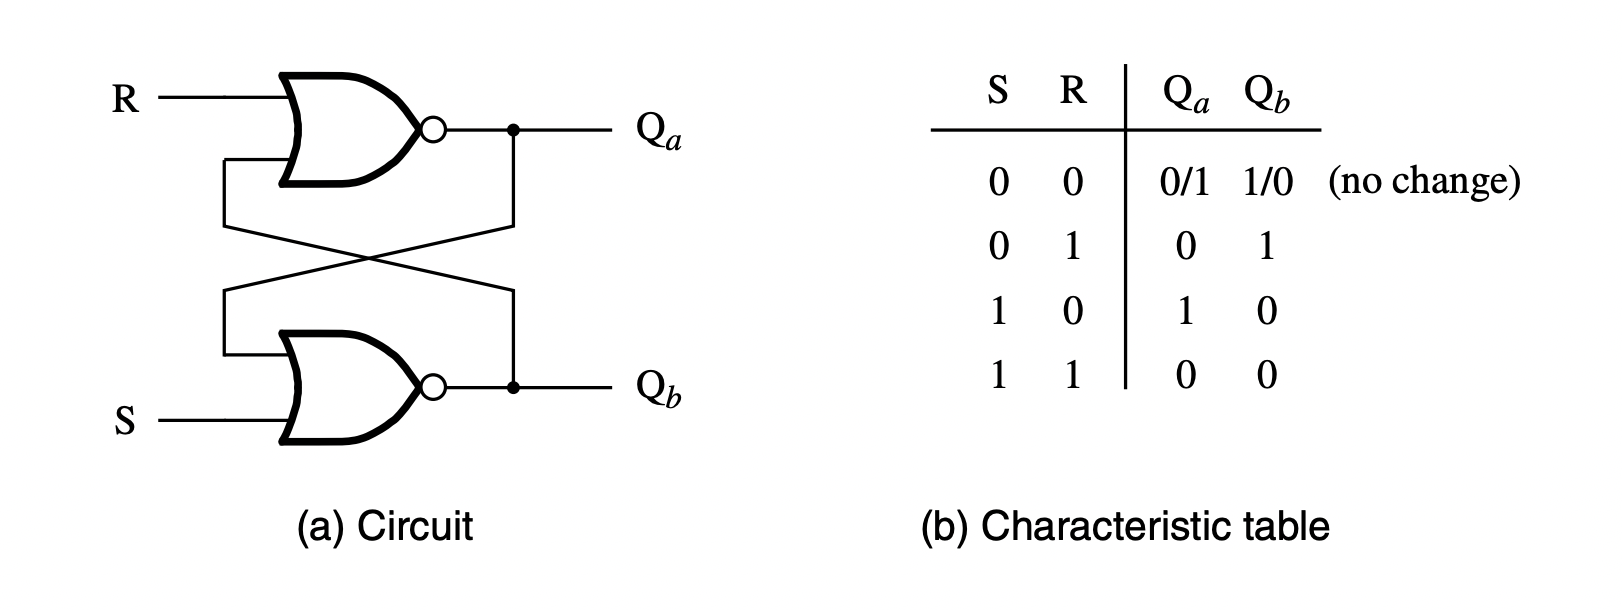
\includegraphics[width=0.7\textwidth]{../media/basicLatch.png}
\caption{Basic Latch}
\label{latch-basic}
\end{figure}
\subsection{Behavior} 
You use $S$ to set the output $Q_a$ to $1$ and $R$ to set $Q_a$ to $0$.

\begin{tabular}{ll|ll}
$S$ & $R$ & $Q_a$ & $Q_b$ \\
\hline
0 & 0 & No change &  \\
0 & 1 & 0 & 1 \\
1 & 0 & 1 & 0 \\
1 & 1 & 0 & 0 \\
\end{tabular}

$S$ functions as the 'set' signal. 


\section{Gated RS Latch}
Add an and gate to the inputs so that you can only enter signals to the latch when 
the $clk$ signal is $1$.

\subsection{Synchronous Reset}
This is when you can only use the reset when the clock is at 1 (basically you just 
AND the $D$ and the $R_n$ for an `active low' reset). Reset behavior is synchronized to the rising edge. 

\subsection{Behavior} 
Same as an RS latch, but you can only send $R$ and $S$ signals when the $clk$ is logic $1$.

\section{Gated D Latch}
Also called `Transparent Latch' or `Level-Sensitive Latch'. 

\subsection{Behavior: } When the clock is $1$, then $Q = D$. $Q$ changes as $D$ changes 
and then when the clock is turned back to $0$, then $Q$ persists in it's last state. 

\section{D Flip-Flops}
\paragraph{Symbol: } Same as the D Latch, but there's a triangle instead of $clk$. If 
it's a \textbf{negative edge} triggered flip-flop, the symbol has a bubble next to the 
clock. \textbf{Positive edge} appears to be the default. 

\paragraph{Edge-Triggered Flip Flop: } The flip flop only changes when the clock is 
on a rising edge or a falling edge. 

\subsection{Master-Slave Flip Flop}
You connect a master D-Latch to a slave D-Latch. The clock signals of one is the inverse 
of the clock symbol going into the other one. 

This setup yields a system where you can only change the value of $Q$ for the slave ($Q_s$) 
on a rising/falling edge. 

\subsection{Behavior} On rising or falling clock edge, the value of $D$ is stored and 
appears in $Q$.

\paragraph{Work-Through demonstration: } Let's say you have the inverted clock going 
to the slave. When you're in logic 1 for the clock, the master is in \textbf{transparent} 
mode. $Q_m = D$. When you switch, the value of the master is stuck and the value of the 
slave is set to $Q_m$. You can't reset the slave value after the transition because the 
\textbf{opaque} mode of the master. 

Pretty cool property! 

\subsection{Why it's Useful}

You can put these in the middle of circuits to save values. Then, you can re-inject inputs 
while you wait for the last half of the circuit to finish processing. It's like splitting 
the circuit into two pieces that can run on different elements simultaneously. 

This is a bit of a dumb way to think about it, but that's the general idea behind how 
they are actually used. 


\section{T Flip-Flop}
Let's take a D Flip Flop component and loop the value of $Q$ and $\bar{Q}$ back to the 
input $D$. Let's make $T$ the new input. $T$ switches the input of $D$ between $Q$ and 
$\bar{Q}$. 

% \section{Flip-Flop Reset/Preset}

% \section{Summary of Objects}

\section{Verilog Implementations}
\subsection{Gated D-Latch}
\begin{lstlisting}
module D_Latch (D, clock, Q, Qb);   
   input D, clock;
   output reg Q, Qb; // `reg` means it's an always block

   always@(D,clock) //defining a block that's sensitive to changes in Q and D.
   begin
      if(clock==1'b1)
      begin // need this begin because you're doing two things in the if block.
         Q = D;
         Qb = ~D;
      end // begin and end function like curly braces in C/C++/Java
   end //if clock == 0'b1, then verilog maintains previous values. 

endmodule
\end{lstlisting}

\subsection{Edge-Triggered Flip Flop}
\begin{lstlisting}
module D_ft(D, clock, Q, Qb)
   input D, clock;
   output reg Q, Qb;

   // Always blocks tell you what you need to 
   always@(posedge clock) // This means you execute this on the positive edge (posedge is a keyword for that)
   begin 
      Q <= D; // use '<=' for describing flip flops.
      Qb <= ~D; // we may get to why in this course but for now it's just a thing...
   end
endmodule
\end{lstlisting}

\subsection{Synchronous Reset (Active Low)}
\begin{lstlisting}
always@(popsedge clock)
begin
   if(resetn == 1'b0)
   begin
      Q <= 1'b0;
      Qb <= 1'b1;
   end
   else 
   begin
      Q <= D;
      Qb <= ~D;
   end
end 

endmodule;

\end{lstlisting}

\chapter{Finite State Machine}
\section{Review}
A finite state machine (FSM) is an object that changes it properties (outputs) 
based on inputs over time. For example, a human could be modeled as a state machine 
where the input is water over time and the output is the need to go to the bathroom. 
\textbf{Sequential circuits} are FSM's.

\subsection{State Diagrams}
\paragraph{Example: } $w$ can be $0, 1$. We are trying to find when $w$ has gone 
$1 \to 0 \to 1$. 
\paragraph{Solution: } We can use a shift register to get all 
the sequential bits of $w$ in, then we use a simple logical expression on the outputs
$w_0 \dot \bar{w_1} \dot w_2$. 

\paragraph{One-Hot Encoding: } When only one of your bits is one. \textbf{one cold} 
is the opposite.

\subsection{Lmao what is an always block actually}
\begin{lstlisting}
always@(A, B, C)
begin

end
\end{lstlisting}
$A, B, C$ are in the sensitivity list, the code inside is `sensitive' to them so 
as they change the internal block is fired. You can only use \textbf{if} statements 
in here. 

\subsection{Case Statements}
Same as in pretty much all other programming languages. 
\begin{lstlisting}
case(A)
   value1:
      do_something;
   value2: 
      do_something_else;
   value3: // multiple lines
      begin
         do_something;
         do_something more;
      end
   default:
      default_behavior;
endcase
\end{lstlisting}

% \subsection{State Machine Diagrams and Sequantial Diagrams}

\subsection{Case Statements for State Machines}
Quick example:
\begin{lstlisting}
module FSM(input w, clock, resetn, output z);
   reg[1:0]y, Y;
   parameter A = 2'b0, B = 2'b01, C = 2'b10, D = 2'b11;
   //state table
   always@(w, y) begin
      case(y) begin
         A: begin
            if(W) 
               Y = B;
            else  
               Y = A;
         end
         B: begin
            if(w)
               Y = B;
            else 
               Y = C;
         end
      endcase
   end

   always@(posedge clk) begin
      if(!resetn)
         y <= A;
      else  
         y <= Y;
   end

   assign z = (y == D);

endmodule
\end{lstlisting}
\begin{itemize}
\item \textit{parameter} lets you define constants. 
\end{itemize}



\chapter{Introduction to Microprocessors}
\section{Computer Organization}
\paragraph{A computer } can read, write, and process data. In order to do so, it has the following main parts:
\begin{enumerate}
\item Input/Output Devices
\item Memory
\item Processor (includes Arithmetic Logic Unit and Control Unit)
\end{enumerate}
All of these are connected through an \textbf{interconnection network}.
\subsection{Memory Unit}
The memory unit can be broken into three main pieces. Overall, it functions to \textbf{store programs} and \textbf{data}. 
\subsubsection{Primary Memory}
\begin{itemize}
\item Stores programs
\item Relatively fast, called `main memory'
\item Made of a collection of \textbf{bit registers}
\end{itemize}
The bit registers in memory are read and written in \textbf{WORDS}. Each word has its own address (consecuitive numbers) and a standardized number 
of bits. 

\subsubsection{Cache}
\begin{itemize}
\item Smaller, faster RAM unit (RAM = Random Access Memory, all can be accessed at the same speed).
\item Holds current parts of a program.
\item Packaged with the processor $\to$ faster to access information from here than from memory.
\end{itemize}

\subsubsection{Secondary Storage}
Basically just external drives.

\subsection{Arithmetic Logic Unit (ALU)}
Most operations are executed here ($+, -, /, \cdot, \leq, \geq, >, <$). Operands are passed here via \textbf{registers}. Registers are 
1 word long and are very fast to access.

\subsection{Control Unit}
Coordinates the rest of the units. Usually distributed throughout the compter. The following main types of operations are coordinated by this unit:
\begin{enumerate}
\item Storing information in memory as programs and data.
\item Moving information to memory for the ALU to process.
\item Moving processed information to the output unit.
\end{enumerate}

\chapter{Basic Concepts in Microprocessors}
\section{Basic Concepts}
\lstset{frame=tb,
  language=verilog,
  aboveskip=3mm,
  belowskip=3mm,
  showstringspaces=false,
  columns=flexible,
  basicstyle={\small\ttfamily},
  numbers=none,
  numberstyle=\tiny\color{gray},
  keywordstyle=\color{blue},
  commentstyle=\color{dkgreen},
  stringstyle=\color{mauve},
  breaklines=true,
  breakatwhitespace=true,
  tabsize=3
}

\begin{lstlisting}
LOAD     R2, LOC     // Copies data from main memory into a register. 
ADD      R4, R2, R3  // R4 = R2 + R3 (contents)
STORE    R4, LOC     // Copies data from a REGISTER to main memory.

MOVE     R2, R4      // Copy contents of R4 to R2
CLEAR    R2          // Set contents of R2 to be 0
ADD      R2, R2, R4  // R2 = R2 + R4
SUB // Same as add but subtraction
MULTIPLY
DIVIDE


AND      R4, R2, R3  // R4 = R2 & R3
OR
NOT
\end{lstlisting}

The processor's \textbf{PROGRAM COUNTER} (PC) holds the address of the next instruction. Each instruction is 1 word in RISC computers.

\section{Memory Locations and Addresses}
1 cell is 1 bit, and n cells is 1 word. Memory is a collection of words, usually from 16-64.
\paragraph{Address spaces: } The possible addresses in a $k$-bit address space range from $0\to 2^{k}-1$
\paragraph{Byte-addressable memory } indexes each byte (8 bits) with an integer $0, 1, 2... n$. Therefore, in a 32-bit word system, 
the address of each word is $0, 4, 8, 12, ...$ in byte addressible memory.

\textbf{Big endian} means that the lower byte address has the more significant digit while \textbf{little endian} holds the oppoiste.

\subsection{Memory Operations}
READ and WRITE are the main operations. 

\begin{itemize}
\item READing copies the contents of a memory location to a processor register. This is done by specifying 
the address in memory that the processor wants to read. 
\item WRITing involves copying the contents of a processor register to a particular 
place in memory. The process sends the address it wishes to write to and the data it wants to write there.
\end{itemize}

\section{Instruction Sequencing}
There are 4 operations needed for running a computer program:
\begin{enumerate}
\item Data transfers between memory and process (READ and WRITE)
\item Arithmetic and logic operators
\item Program sequencing and control (branching, subroutines, etc.)
\item Input and Output
\end{enumerate}

\subsection{RISC and CISC Instructions}
\paragraph{RISC: } Each instruction is 1 word long. All arguments must be in registers already.
\paragraph{CISC: } Each instruction can be $\geq$ 1 word long. This enables more complex operations.

\section{Branching}
So far we have talked about \textbf{straight line sequencing}. Instructions are executed in the exact order they are written. But what 
if we want to loop?

\begin{lstlisting}
// Some computation
BGT      R4, R5, LOOP      // Go to LOOP if R4 > R5
// Stuff to be executed if R4 <= R5...

LOOP:
   // To be executed if R4 > R5

// SIDE NOTE: This is how you use constants:
SUBTRACT R2, R2, #1 // R2 = R2 - 1
\end{lstlisting}

\section{Addressing Modes}
% So far we have used register modes ($R2$) and absolute modes ($#1$). 
A register holding the address of some information in memory is a \textbf{pointer}. Using pointers is called 
the \textit{indirect addressing mode}. 
\begin{lstlisting}
LOAD     R2, R5         // Loads the stuff from the MEMORY ADDRESS that R5 holds into R2.
MOVE     R2, R5         // Puts the IMMEDIATE VALUE held in R5 into R2.
MOVE     R2, #300       // R2 = 300;
CLEAR    R2             // CLEARS R2 to 0's.

ADD      R4, R0, #200   // R0 usually holds 0's. This what MOVE really does.
\end{lstlisting}

\paragraph{Index mode } of addressing is when you use an address register to hold the address of the first word in a list. 
\begin{lstlisting}
// Memory address is equal to some value X (let's say address #96 in memory) plus a register value at Ri 
X(Ri) // This is how you address that memory address.
\end{lstlisting}

\section{More on Assembly}
\begin{lstlisting}
TWENTY   EQU   20 // Whenever the assembler sees `TWENTY' it will be replaced by 20.

ORIGIN   100      // Inser this at the beginning of a block to specify that code below should be placed in memory starting at address #100

SUM   :  Reserve  4  // 4-byte space reserved @ address 100
N     :  Dataword    // N = #150 @ address 204
End // ends the program.

%10110101 // how to specify numbers in binary 
0x5f      // hot to specify number in hex
\end{lstlisting}

\section{Stacks}
Same common datastructure we ran into before in CSC190. Only one end can be read/added to, and it's LIFO (last in, first out).

\paragraph{The Stack Pointer (SP)} points to the address of the end of the stack (Processor stack). Common practice: stack grows in direction of 
\textit{decreasing memory addresses}. 
The push operation works as follows (pushing word in $R_i$):
\begin{lstlisting}
SUB         SP, SP, #4     // Decrementing stack pointer by 4 bytes (1 word).
STORE       Ri, SP
// Now the pop operator:
LOAD        Ri, SP
ADD         SP, SP, #4
\end{lstlisting}

\section{Subroutines}
Same as a function. Uses branching, but it knows that it has to return to where it was called from. We use the \textbf{RETURN} command 
to return to the calling place. The address of the calling place is stored in the \textbf{LINK REGISTER}.

\begin{lstlisting}
CALL        FUNCNAME       // Stores current PROGRAM COUNTER in LINK REGISTER, branches to subroutine.
// .. some code ..
FUNCNAME: 
   // .. some code ..
   RETURN                  // Branches back to address stored in LINK REGISTER
\end{lstlisting}

\subsection{Subroutine Nesting}
If you call a function in a function, the LINK REGISTER can only hold one address at a time. Since we need LIFO structure to 
tell us where to branch back to at each successive return, we use the \textbf{PROCESSOR STACK} to store the further addresses.

\paragraph{Process for calling a nested function: }
\begin{enumerate}
\item Return address in LR $\to$ PROCESSOR STACK @SP.
\item Store current address in LR and branch to the next function.
\item When you return from the nested function, transfer the original LR pointer back from PROCESSOR STACK @SP.
\item Return as normal to address in LR when you're done with the original subroutine.
\end{enumerate}

\subsection{Parameter Passing}
This can be done with registers or via the \textbf{PROCESSOR STACK}. Here are the steps for the PROCESSOR STACK approach:
\begin{enumerate}
\item Push the arguments you want to pass to the stack in the caller.
\item Once in the subroutine, save the contents of current registers to the stack to preserve the state of the calling program.
\item Use an offset equal to the number of SAVED REGISTERS to access passed variables.
\item Carry out the subroutine.
\item Restore the disturbed registers from the stack (pop them off).
\item Branch back to the address of the caller and re-establish the SP to what it was originally.
\end{enumerate}

\subsection{Stack Frame}
\paragraph{Definition: } The Stack Frame is the space allocated to a subroutine when it is called. It is useful to 
have a \textbf{FRAME POINTER} that points to just above the PASSED PARAMETERS (unlike the STACK POINTER SP that points 
to the actual top of the stack that also holds the saved registers). 

\paragraph{FRAME POINTER FP } is a constant for the duration of the subroutine program. It is equal to the STACK POINTER SP 
at the beginning of the subroutine call.

\section{Flags and Conditionals}
You pretty much always want to branch/call a subroutine on a conditional. Here's who they work:
\subsection{Comparisons}
\textbf{CMP R2, R1} lets you compare the values of two things. It performs the operation $R2 - R1$ and stores attributes of the result in global \textbf{FLAGS}
\subsection{Flags}
Flags are values you can use to branch. They store attributes of the previous comparison or operation.
\begin{enumerate}
\item $N$: If the result was negative.
\item $Z$: If the result was zero.
\item $C$: If the result of an unsigned operation overflows. 
\item $V$: If the result of a signed operation overflows.
\end{enumerate}

The following Assembly directives make use of the previous comparison's flags:
\begin{enumerate}
\item $BEQ$: If the previous comparison yielded equality.
\item $BLT$: If the previous comparison yielded less than.
\item $BGT$: If the previous comparison yielded greater than.
\end{enumerate}



\chapter{IO Devices}
You access IO devices in the same way you might access regular registers. The \textbf{device interface} gives you a few registers that 
allow you to communicate:
\begin{enumerate}
\item Data
\item Status
\item Control
\end{enumerate}

\section{Program Control IO}
You use a program called a \textbf{Program Control Interface} to write and control an IO device. 

Because the processor, input, and output devices may work at different rates, you need to wait for a response to any signal you 
send to one to make sure it's ready for the next one. These are called \textbf{STATUS FLAGS}, and reading them is called \textbf{POLLING}. 


\section{Interrupts}
You can use the infinite loop approach where you just keep POLLING the STATUS FLAG of an IO device until it's ready. That takes a lot of 
compute power and you can't do anything during the wait time, which is a problem.

\paragraph{INTERRUPT SERVICE ROUTINE } is called by an interrupt signal from an IO device. Here is the processor's steps for dealing with one.
\begin{enumerate}
\item The processor finishes instruction $i$ that it is in the middle of.
\item The processor branches to the INTERRUPT ROUTINE. PC $\to$ PROCESSOR STACK.
\item The INTERRUPT ROUTINE is executed.
\item The PC is restored from the PROCESSOR STACK.
\end{enumerate}

\subsection{Notes on SUBROUTINE INTERRUPT IMPLEMENTATION: } 
At the beginning of the subroutine, the processor must send an \textbf{INTERRUPT ACKNOWLEDGE} make sure that, when the subroutine RETURNS, 
an infinite loop does not occur. Alternatively, the successful execution of the subroutine can implicitly notify the IO device.

\paragraph{REGISTERS MUST BE RESTORED } because you don't know when the interrupt subroutine will be executed. It could be in the middle of another 
very sensitive subroutine. 

\subsection{Enable and Disabling Interrupts} 
Sometimes you don't want to branch away from the main progam. Therefore, the processor has some STATUS REGISTERS PS that have a bit INTERRUPT INABLE IE 
that, when set to 0, disable interrupts.

\textbf{You must set this } to 0 while inside the subroutine to avoid an infinite loop.. 

\paragraph{IO MODE } bit in the control interface of the IO device can also allow you to set whether it sends interrupts or not.

\subsection{Process for a Single Device Interrupt Call}
\begin{enumerate}
\item Device raises interrupt
\item Processor branches to the interrupt subroutine
\item STATUS REGISTER PS is saved to the stack, along with the PROGRAM COUNTER PC.
\item STATUS REGISTER PS has INTERRUPT ENABLE IE that is set to 0. 
\item Subroutine runs.
\item STATUS REGISTER PS is restored from the saved version. 
\end{enumerate}

\section{Multiple Device Interrupts}
The above system works fine when you just have one interrupt at a time or one device performing the interrupts. 

\subsection{Approach One: Naïve Polling}
You can just do the same thing as before, just executing the interrupts in the order you poll them if they happen to come at the same time. However, 
polling takes time.

\subsection{Vectored Inputs}
If you allow the interruptor to send a message along with their interrupt, you can have code in the processor that tells it how to 
interpret the signal.

\paragraph{INTERRUPT VECTOR TABLE } is stored (usually in the lowest address range). The information in a vectored interrupt contains the 
address of one of the vectors in that table. The contents of that vector in the table is the address of the interrupt subroutine.

\subsection{Interrupt Nesting}
If an interrupt comes in while executing another interrupt's subroutine, there's a chance that it will be of higher priority. Therefore, 
we need an interrupt priority system.

\paragraph{PROCESSOR PRIORITY } is the priority of the current process. Only interrupts with a higher priority are executed. Priority is
communicated in the interrupt vector. 

\section{Processor Control Register}
We already know that the INTERRUPT ENABLE IE bit is in the PROCESSOR STATUS register which is one of the PROCESSOR CONTROL REGISTERS.

IPS is where PS is saved automatically at the start of an interrupt. PS is autorestored from here at the end.

IENABLE register enables device specific INTERRUPT ENABLE bits. 

IPENDING register shows which interrupts are active. 

Since all registers are 1 word long, you can generally have 32 IO devices. 

In order to read and write from PROCESSOR CONTROL REGISTERS, you treat them like regular registers. 

\chapter{Closing Remarks}
\section{Multiplexer Synethesis}
You can make any logical circuit out of a bunch of multiplexers. The naïve aproach is to have the actual inputs of the 
multiplexer be constants and the selector inputs be your inputs to the function. 

\paragraph{Shannon's Expansion } allows you to further simplify your naïve multiplexer layout:
$$f(w_1, ... , w_n) = \bar{w}_1\cdot f(0, w_2, ..., w_n) + w_1 \cdot f(1, w_2, ..., w_n)$$

\section{Timing Considerations for Flip Flop Circuits}
We need to know $F_{max}$, the maximum frequency at which we can run our clocks when using a flip flop.

\paragraph{Hold time violation } is 
\paragraph{Timing parameters } 
\begin{itemize}
\item $t_{su}$: \textbf{Set up time} while data D must be stable for a D-latch or D-fip flop. 
\item $t_h$: Data must stay stable during \textbf{hold time}
\item $t_{cQ}$: Time from \textbf{clock signal to Q} for a flip flop.
\end{itemize}

\paragraph{To get clock's $T_{min}$}, you add up the maximum required time for a signal to propagate through the circuit. 

\subsection{Clock Skew}
Clock signal might not arrive at different flip flops at the same time. 

\paragraph{$t_{skew}$} = time of arrival at sink - time of arrival at source.

If skew time is positive, you can have a higher $F_max$. Negative leads to lower $F_max$. 

\subsection{Process for Timing Analysis}
\begin{enumerate}
\item Calculate longest path the signal must traverse during a clock cycle. $T_{min} \geq T_{longest_path}$
\item Calculate hold time violation (which is the time the data must be constant for the latch to `save' the data). `'
\item Calculate time violation: 
\end{enumerate}

\end{document}
